\chapter{Injecting an informational reward}
\begin{quotation}
\noindent ``\emph{The ideal of behaviourism is to eliminate coercion: to apply
	controls by changing the environment in such a way as to reinforce the
	kind of behaviour that benefits everyone.}''
\begin{flushright}\textbf{Burrhus Frederic Skinner}\end{flushright}
\end{quotation}
\vspace*{0.5cm}


We have described in section \ref{section:problems_1_timestep_reward} why
a 1-per-timestep reward structure led to an undesired behaviour of laziness,
in which the agent only maximised its reward on the last episode of its
training trials.\\

We introduce a simple, yet effective way to allow problems with similar 
reward structures to be meta-learned. In hand-designed strategies aimed to
solve such problems, the designer holds the implicit knowledge that a short
episode is a bad thing, and treats the reward streams of each episode 
separately. In meta-learning, just like we feed back a termination flag, which
is not an environment-level value but rather a "process-level" value (where
the process is the training process we replicate in a trial); we can
introduce a process-level reward to give information to the agent 
performing the trial.\\

We propose to add a small negative reward at the end of each episode, 
interrupting the continuous reward stream to force the agent to perform
well for each of the episodes in the trial.\\

Our agent is trained on the training set of 20 permutations listed on table
\ref{tab:20perms}, on trials of 3 episodes. The reward for the last 
timestep of each episode is set to -10. Figure \ref{fig:magic} shows how
the episode-wise reward curve evolves during training. We see that all
three episodes reach a high reward, but more importantly, performance
increases for the second and third episode. \\

This is clearer on Figure~\ref{fig:magic_rewards}, where we see
that episodes 2 and 3 get a higher average than episode 1. We also see
however that letting the agent play beyond its training horizon leads to
a generally lower average reward. A second surprise is the fact that the
average reward for the third episode when testing on unseen permutations is
below the average reward of second episodes. It is however still above the average
reward for first episodes. We suspect this variance in the results is due
to the closeness in performance of all three episodes.\\

\begin{figure}
	\centering
	\subfloat[][Full training graph]{
		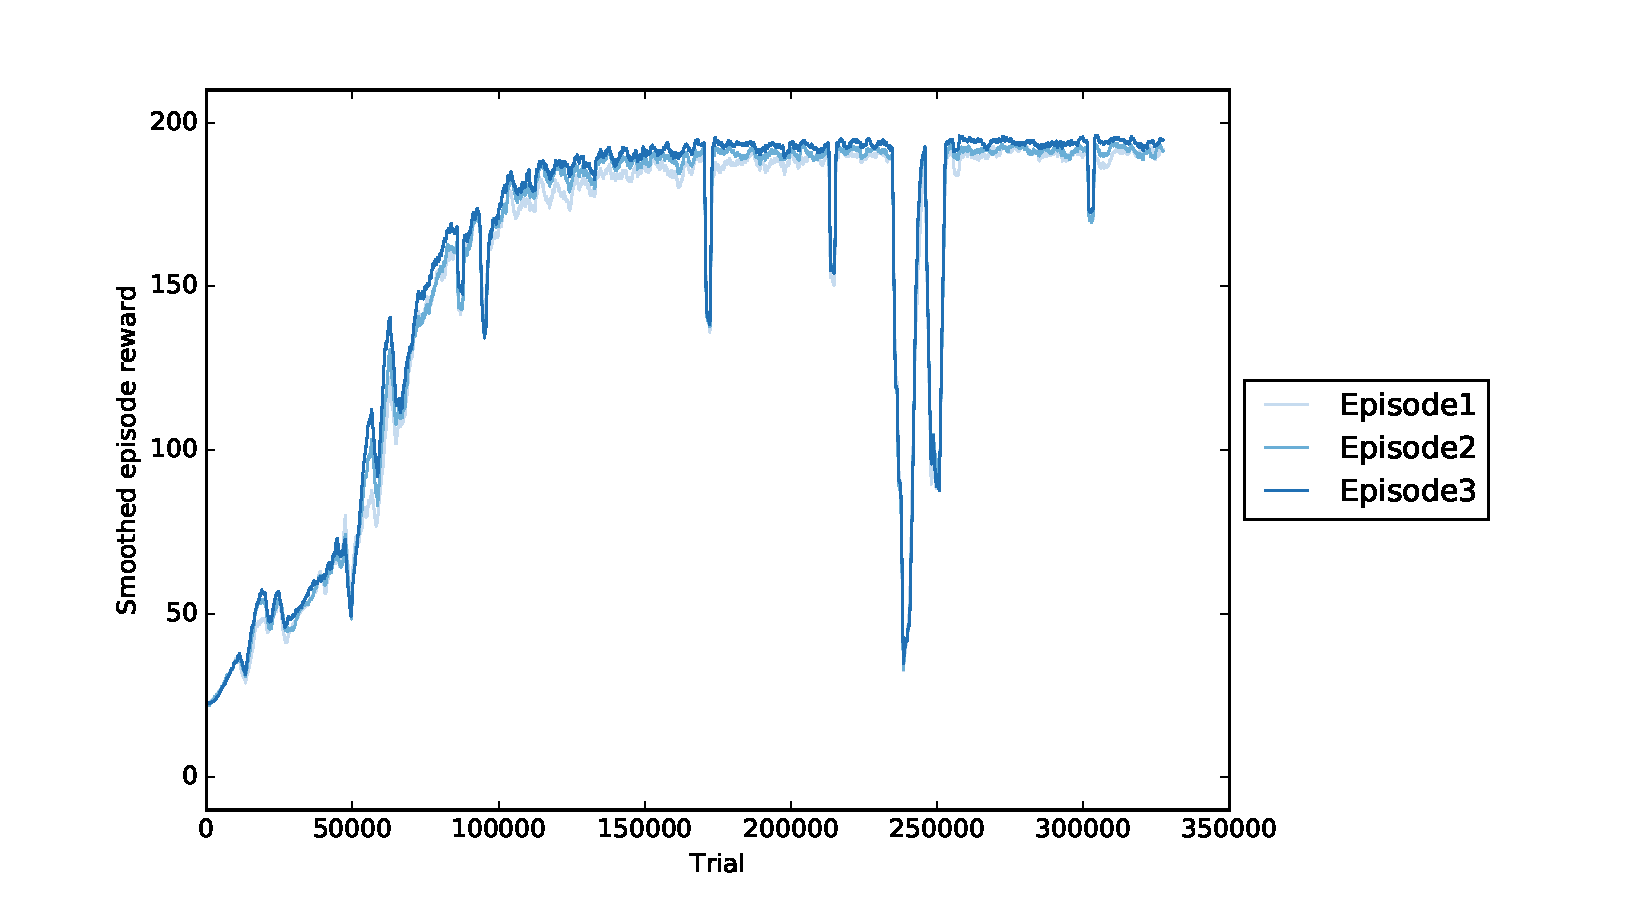
\includegraphics[width=0.8\linewidth]{fig/res_magic_neg10.pdf}}\\
	\subfloat[][Close-up of the last trials]{
		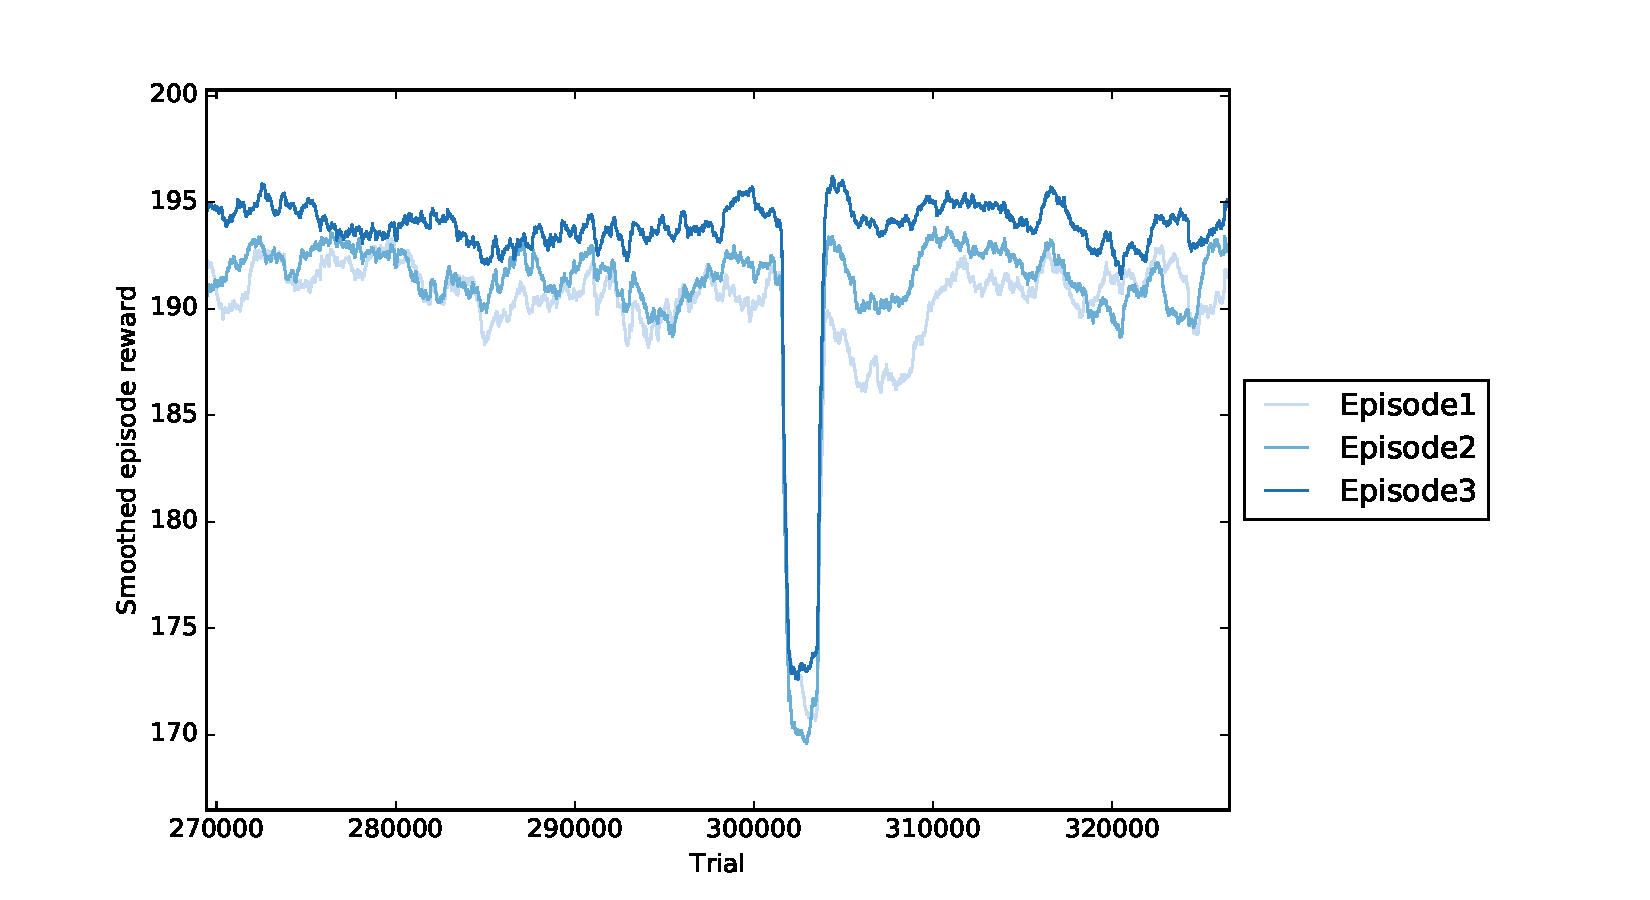
\includegraphics[width=0.8\linewidth]{fig/res_magic_neg10_closeup.pdf}}
	\caption{Episode-wise reward evolution during the training of an
	agent playing trials of 3 episodes with a small negative reward
	at the end of each episode.}
	\label{fig:magic}
\end{figure}

\begin{figure}
	\centering
	\subfloat[][Training permutations]{
		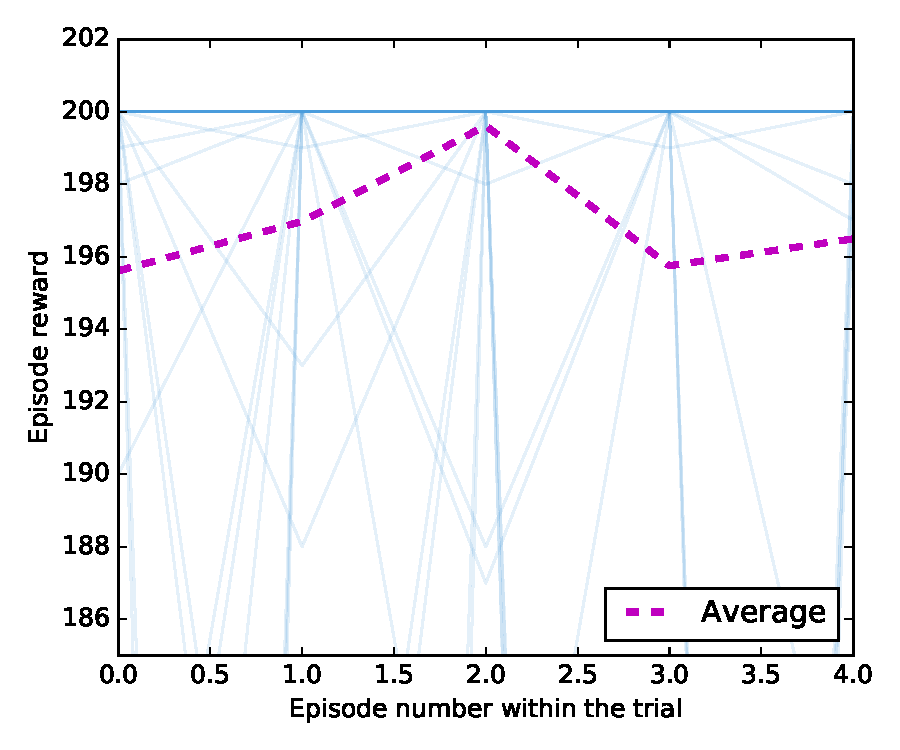
\includegraphics[width=0.45\linewidth]{fig/magic_rewards.pdf}}
	\subfloat[][Testing permutations]{
		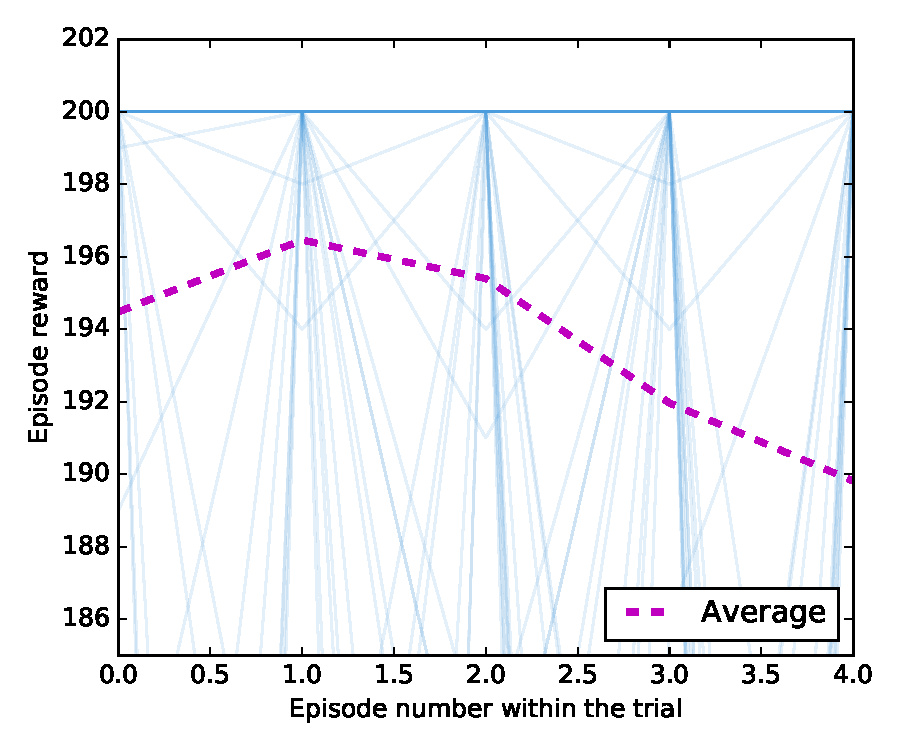
\includegraphics[width=0.45\linewidth]{fig/magic_rewards_unseen.pdf}}
	\caption{Testing performance of the agent trained with the reward
	injection. Several runs are displayed in blue on the same plot, and their
	average is shown as a red dashed line.}
	\label{fig:magic_rewards}
\end{figure}

Even though this is a success, we think there might be a better solution for
problems with a similar reward structure. For example, Wang et al.
\cite{learningtorl} present an experiment (bandits with dependent arms II) 
where the optimal long-term strategy is to start by playing a suboptimal action
voluntarily to gain information that will then allow the agent to play
optimal moves in future episodes. The setting of our experiment doesn't lend
itself to the obligation of abandoning short-term reward for a higher long-term
reward, but adapting it to make room for that type of experiment could be
an interesting lead to follow in future work.\\

We are aware that the results shown so far could seem like they miss one 
of the key promises of meta-learning that were made in the introduction :
the \todo{what promise?} Indeed,
one could argue that meta-learning is not really needed in the setting
presented in this chapter as the average reward for the first episode is 
already almost optimal. This is why we propose to test the exact same agent
that was used in the experiments of Figures~\ref{fig:magic} and 
\ref{fig:magic_rewards} for a different CartPole game it has 
actually never been trained to play by inverting one parameter : the reward.
For this experiment, we start giving the agent a reward of +1 at every timestep
only from the moment at which the environment considers it has failed the
episode, until the end of the 200-timesteps episode. 
To our surprise, and perhaps we should emphasize this : 
\textbf{without having been retrained}, the agent learns to fail as quickly
as it can after the first episode. Figure~\ref{fig:magic_magic} shows this
result.

\begin{figure}
	\centering
	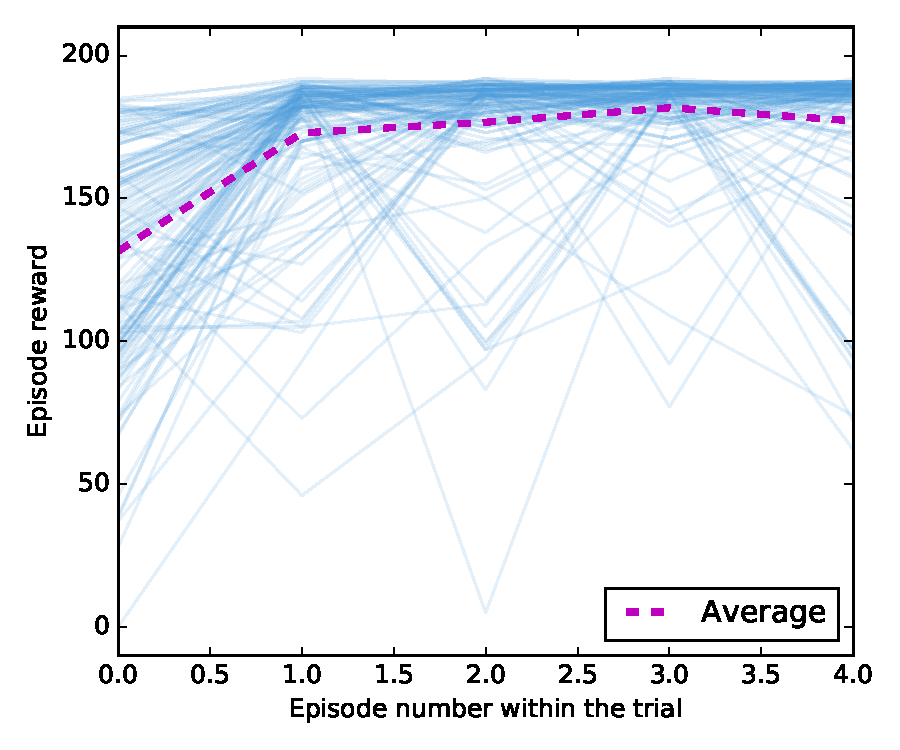
\includegraphics[width=0.8\linewidth]{fig/magic_magic.pdf}
	\caption{Reward per episode for an agent trained to balance the pole,
	tested on a task where a reward is generated as soon as it fails at
	doing what it was trained to do. Each different run is shown in light
	blue; the average of all runs is shown as a dashed red line.}
	\label{fig:magic_magic}
\end{figure}

\subsubsection{Summary}
In this section, we have proposed and successfully tested injecting an
informative process-level negative reward at the end of each episode, 
indicating to the outer algorithm that it should try to keep each episode
running for as long as possible. We trained an agent using this injected
reward on trials of 3 episodes and found that it performed well on each
episode, but that performance generally increased between episodes.\\

We also tested this agent on a completely new problem, where it was implicitly
asked to fail at what it had been trained for as quick as possible. The results
showed that the agent quickly learned to fail after the first episode, increasing
dramatically its average reward over following episodes.





